\documentclass{article}

\usepackage{fancyhdr}
\usepackage{lastpage}
\usepackage{extramarks}
\usepackage[usenames,dvipsnames]{color}
\usepackage{amsmath}
\usepackage{amsthm}
\usepackage{amsfonts}
\usepackage{changepage}
\usepackage{lineno}
\usepackage{algpseudocode}
\usepackage{graphicx}

\topmargin=-0.45in
\evensidemargin=0in
\oddsidemargin=0in
\textwidth=6.5in
\textheight=9.0in
\headsep=0.25in

\linespread{1.1}

\pagestyle{fancy}
\lhead{\hmwkAuthorName}
\chead{\hmwkClass\ (\hmwkClassInstructor\ \hmwkClassTime): \hmwkTitle}
\rhead{\firstxmark}
\lfoot{\lastxmark}
\cfoot{}
\renewcommand\headrulewidth{0.4pt}
\renewcommand\footrulewidth{0.4pt}

\setlength\parindent{0pt}

\newcommand{\enterProblemHeader}[1]{
    \nobreak\extramarks{}{Problem \arabic{#1} continued on next page\ldots}\nobreak{}
    \nobreak\extramarks{Problem \arabic{#1} (continued)}{Problem \arabic{#1} continued on next page\ldots}\nobreak{}
}

\newcommand{\exitProblemHeader}[1]{
    \nobreak\extramarks{Problem \arabic{#1} (continued)}{Problem \arabic{#1} continued on next page\ldots}\nobreak{}
    \stepcounter{#1}
    \nobreak\extramarks{Problem \arabic{#1}}{}\nobreak{}
}

\setcounter{secnumdepth}{0}
\newcounter{homeworkProblemCounter}
\setcounter{homeworkProblemCounter}{1}
\nobreak\extramarks{Problem \arabic{homeworkProblemCounter}}{}\nobreak{}

\newenvironment{homeworkProblem}{
    \section{Problem \arabic{homeworkProblemCounter}}
    \enterProblemHeader{homeworkProblemCounter}
}{
    \exitProblemHeader{homeworkProblemCounter}
}

\newcommand{\hmwkTitle}{Homework\ \#1}
\newcommand{\hmwkDueDate}{September 11, 2013 at 4:30pm}
\newcommand{\hmwkClass}{CS311}
\newcommand{\hmwkClassTime}{Section 3}
\newcommand{\hmwkClassInstructor}{Professor Lathrop}
\newcommand{\hmwkAuthorName}{Josh Davis}

\title{
    \vspace{2in}
    \textmd{\textbf{\hmwkClass:\ \hmwkTitle}}\\
    \normalsize\vspace{0.1in}\small{Due\ on\ \hmwkDueDate}\\
    \vspace{0.1in}\large{\textit{\hmwkClassInstructor\ \hmwkClassTime}}
    \vspace{3in}
}

\author{\textbf{\hmwkAuthorName}}
\date{}

\begin{document}

\maketitle

\pagebreak

\begin{homeworkProblem}
    Demonstrate that the quicksort implementation given is incorrect by
    providing an input on which the algorithm does not produce correctly sorted
    input. Briefly explain why the input fails.
    \\

    \textbf{Solution}

    The following input \(list = [3, 3]\), \(start = 0\), and \(end = 1\), will
    cause the given implementation of quicksort to loop infinitely.
    \\

    \textbf{Explanation}

    The reason this input fails is because when the first call to \(partition\)
    happens, \(left = start + 1 = 1\) and \(right = 1\). The \(while\) loop on
    line 3 waits until \(left \leq right\).
    \\

    However, \(left\) and \(right\) can never advance past each other because
    neither line 4 or 7 take into the account the possibility when the pivot
    value equals either \(list[left]\) or \(list[right]\).  To fix this, all we
    need to do is change line 4 to be less than \textbf{or equal}, \(list[left]
    \leq list[start]\). Now \(left\) can be incremented and cause the \(while\)
    loop to finish.
    \\

    There is one last issue. When \(partition\) returns, it will set \(mid
    = 1\). The problem though is that we recursively call \(quicksort\) on
    \(start = 0\) and \(end = 1\). Which is the exact same as the first call
    that we made to \(quicksort\).  To fix this, the first call to
    \(quicksort\) should pass \(mid - 1\) instead of \(mid\).
    \\

    This is what the final code should look like:

    \begin{linenumbers}[1]
        \renewcommand\linenumberfont{\normalfont\bfseries\small}
        \begin{algorithmic}
            \Function{Quick-Sort}{$list, start, end$}
                \If{$start \geq end$}
                    \State{} \Return{}
                \EndIf{}
                \State{} $mid \gets \Call{Partition}{list, start, end}$
                \State{} \Call{Quick-Sort}{$list, start, mid - 1$}
                \State{} \Call{Quick-Sort}{$list, mid + 1, end$}
            \EndFunction{}
        \end{algorithmic}
    \end{linenumbers}

    and:

    \begin{linenumbers}[1]
        \renewcommand\linenumberfont{\normalfont\bfseries\small}
        \begin{algorithmic}
            \Function{Partition}{$list, start, end$}
                \State{} $left \gets start + 1$
                \State{} $right \gets end$
                \While{$left \leq right$}
                    \While{$left \leq end \wedge list[left] \leq list[start]$}
                        \State{} $left \gets left + 1$
                    \EndWhile{}
                    \While{$right \geq start \wedge list[right] > list[start]$}
                        \State{} $right \gets right - 1$
                    \EndWhile{}
                    \If{$left \leq right$}
                        \State{} \Call{swap}{$list, left, right$}
                    \EndIf{}
                \EndWhile{}
                \State{} \Call{swap}{$list, start, right$}
                \State{} \Return{} $right$
            \EndFunction{}
        \end{algorithmic}
    \end{linenumbers}

\end{homeworkProblem}

\pagebreak

\begin{homeworkProblem}
    Solve the following parts of the problem using double pole or single pole
    switches.
    \\

    \textbf{Part A}

    Draw a diagram that controls a single light with two switches.
    \\

    \begin{figure}[h]
        \centering

        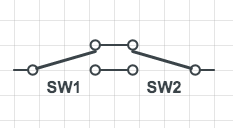
\includegraphics[scale=.5]{circuitA.png}

        \caption{Circuit with two switches}
        \label{fig:circuitA}
    \end{figure}

    \textbf{Part B}

    Draw a diagram that controls a single light with three switches.

    \begin{figure}[h]
        \centering

        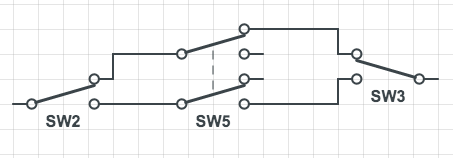
\includegraphics[scale=.5]{circuitB.png}

        \caption{Circuit with three switches}
        \label{fig:circuitB}
    \end{figure}

    \textbf{Part C}
    Describe for \(n > 3\) an electrical circuit with a single light controlled
    by \(n\) switches.
    \\

    \textbf{Solution}
    For \(n > 3\), all you need to do is add more switches between the two ending
    single pole, double throw switches. By connecting the ends of the dpdt to
    opposite ends of the preceeding dpdt, you'll ensure there will always be a
    connecting regardless of whether the switch is on or off.

    \begin{figure}[h]
        \centering

        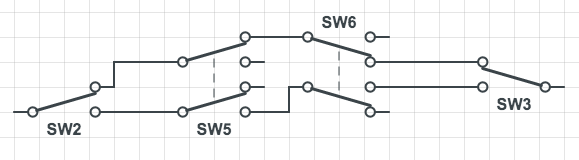
\includegraphics[scale=.5]{circuitD.png}

        \caption{Circuit with four switches}
        \label{fig:circuitD}
    \end{figure}

    \pagebreak

    \textbf{Part D}
    Prove it using induction for all \(n > 3\).

    \begin{proof}
        We will prove that a single light switch can be toggled using \(n\)
        number of switches where \(n > 3\).
        \\

        \textbf{Base} The base case that we need to prove is for when \(n = 4\).
        By looking at Figure ~\ref{fig:circuitD}, it can be seen that whatever
        position the 4 switches are in, the circuit is always only one switch
        away from either being broken or connected for all switches.
        \\

        \textbf{Step} The step case we must prove that given \(n\) is a valid circuit
        that fits our criteria, by adding one more switch, \(n + 1\) switches, we
        can still toggle the light from all \(n\) switches.
        \\

        Consider a circuit with \(n\) switches. To create a circuit with \(n +
        1\) switches, we can do so by adding one more switch into the circuit.
        \\

        By the induction hypothesis, we know that a circuit with \(n\) switches
        allows each switch to toggle the light. In order to satisfy the adding
        of a new switch, we must ensure that when adding our new switch, the
        connection can always be completed through one of the paths.
        \\

        If our circuit looks like the switch in Figure ~\ref{fig:circuitD}, except
        with \(n\) switches, we can take a new dpdt switch and connect it's top
        incoming switch to the previous dpdt switch's top output. Then we take
        the very bottom output of the previous dpdt and hook it up to the
        bottom input.  \\

        It's easy to see that toggling the newly added switch will just result
        in breaking one circuit while completing another circuit, thus toggling
        the lightbulb. Thus this means our circuit now has \(n + 1\) switches
        and our proof is complete.
    \end{proof}
\end{homeworkProblem}

\pagebreak

\begin{homeworkProblem}
    Using the implemenation of insertion sort given, solve the following problems.
    \\

    \textbf{Part A}

    Identify a useful invariant \(I_0\) for the outer loop, that is, a loop
    invariant which will allow you to complete parts \(b\) through \(d\).
    \\

    \textbf{Solution}

    The loop invariant will be the following:

    \begin{adjustwidth}{2.5em}{0pt}
        When looping, all of the original elements in \(list[0 \hdots i - 1]\)
        will still be there but will be in sorted order.
        \\
    \end{adjustwidth}

    \textbf{Part B}

    Prove that if \(I_0\) holds after the last iteration of the outer loop
    completes, then the algorithm sorts \(list\) in ascending order.

    \begin{proof}
        We will prove that \(I_0\) holds after the last iteration and that the
        array is sorted.
        \\

        The \(for\) loop in the code iterates from \(i = 1\) all the way up to
        \(list.length\). When the \(for\) loop terminates, \(i = list.length\),
        which will mean that \(list[0 \hdots i - 1]\) will consist of the first
        \(i\) elements in the array in sorted order.
        \\

        Since the range contains the whole array, it is obvious that all of
        \(A\) will now be sorted, which concludes the proof and the
        \textbf{Termination} part of the loop invariant.
    \end{proof}

    \textbf{Part C}

    Prove that \(I_0\) holds before the loop is executed for the first time.

    \begin{proof}
        We will prove that \(I_0\) holds before the loop is executed for the
        first time.
        \\

        The \(for\) loop in the code iterates from \(i = 1\) all the way up to
        \(list.length\). When the \(for\) loop starts, \(i = 1\), which will
        mean that \(list[0 \hdots i - 1]\) will consist of just \(list[0 \hdots 0]\)
        elements, or one element.
        \\

        This is trivial because any range with one element is always sorted. This
        concludes the proof and the \textbf{Initialization} part of the loop
        invariant.
    \end{proof}

    \textbf{Part D}

    Prove that \(I_0\) is an invariant for the outer loop.

    \begin{proof}
        To prove that \(I_0\) is an invariant for the \textbf{Maintenance}
        step, we'll have to prove that lines 4--7 are also correct by using
        another loop invariant.
        \\

        The inner loop invariant, \(I_1\), will be as follows:

        \begin{adjustwidth}{2.5em}{0pt}

            Each iteration the elements in the range \(list[j \hdots i]\) will be
            greater or equal to the value \(v\).
            \\

            \textbf{Initialization}

            At the beginning of the loop, \(j = i\) (line 3). Which means that
            the range consists of the elements \(list[i \hdots i]\), or just
            one element. Since \(v\) is initialized to be equal to \(list[i]\),
            trivially, any value is always greater or equal to itself. Thus the
            invariant holds.
            \\

            \textbf{Maintenance}

            During each iteration of the loop, the value of \(list[j - 1]\)
            is moved to the position \(list[j]\) because of line 5.  The value
            of \(j\) is then decremented by one because of line 6.
            \\

            This now means that \(list[j]\) and \(list[j - 1]\) contain the
            same value. This is important because it maintains the loop
            invariant, \(I_1\). Since \(list[j]\) and \(list[j - 1]\) are in
            ascending order the loop invariant holds because all the elements
            in the range \(list[j \hdots i]\) are in ascending order as well.
            Thus the loop invariant holds.
            \\

            \textbf{Termination}

            The while loop ends either when \(j \leq 0\) or \(list[j - 1] \leq
            v\).
            \\

            In the first case, when \(j = 0\), this would mean that every value
            in \(list[0 \hdots i]\) is greater than or equal to \(v\).
            Therefore there can be no element that could be less than \(v\)
            since 0 is the beginning of the list. Thus the loop invariant
            holds.
            \\

            In the second case, when \(list[j - 1] \leq v\), it means that
            \(list[j \hdots i]\) is all greater than or equal to \(v\) because
            if the value \(list[j - 1]\) were to be in the range, the loop
            invariant would no longer hold. Thus the loop invariant holds.
        \end{adjustwidth}

        Now that we can see that the loop invariant \(I_1\) is correct we can
        now continue with the \(I_0\) invariant.
        \\

        According to the loop invariant \(I_1\), we can see that every value
        \(list[j \hdots i]\) is greater or equal to \(v\). We know that all
        values from \(list[0 \hdots j - 1]\) are the original elements but in
        sorted order. By inserting \(v\) into the position \(list[j]\) on line
        8, we are placing \(v\) into a spot such that all values \(list[0] \leq
        list[1] \hdots list[j - 2] \leq list[j - q] \leq v\) and \(v < list[j +
        1] \leq list[j + 2] \hdots list[i - 1] \leq list[i]\).
        \\

        Therefore we have proven the \textbf{Maintenance} step of the loop invariant
        \(I_0\) with the help of the other loop invariant, \(I_1\). Thus this
        concludes our proof.
    \end{proof}
\end{homeworkProblem}

\pagebreak

\begin{homeworkProblem}
    Prove or disprove \( (A - B) \cup C = (A \cup B) - C \).
    \\

    \textbf{Counterexample}

    Let \(A = \emptyset \), \(B = \emptyset \) and
    \(C = \left\{ {1}\right\} \). Which gives this for the left hand side:

    \[
        (A - B) \cup C = (\emptyset - \emptyset) \cup \left\{ 1 \right\} = \emptyset \cup \left\{ 1 \right\} = \left\{ 1 \right\}
    \]

    And the right hand side:

    \[
        (A \cup B) - C = (\emptyset \cup \emptyset) - \left\{ 1 \right\} = \emptyset - \left\{ 1 \right\} = \emptyset
    \]

    Since the left doesn't equal the right, the proposition has been disproven.
\end{homeworkProblem}

\begin{homeworkProblem}
    Given an instance of the longest common subsequence problem.

    \textbf{Solution}

    Given two strings, \(s = ``abcdefg"\) and \(t = ``biczdxyg"\), the longest
    common subsequence between the two is \(``bcdg"\).
\end{homeworkProblem}

\begin{homeworkProblem}
    One hundred quarters lie scattered about on a table before you. Some known
    n of them are heads up, while the rest are tails up. You cannot in any way
    observe the configuration of individual quarters (perhaps you are
    blindfolded). You can, however, pick them up and place them back on the
    table in the opposite configuration, ie flip them.
    \\

    Your objective is to
    divide the one hundred quarters into two groups such that each group has
    the same number of heads. The two groups need not have the same number of
    quarters. How do you do this?
    \\

    \textbf{Solution}

    Given the number of coins is 100, we can get the same number of quarters in
    both groups by splitting the quarters into two groups of 50. Since there
    are \(n\) heads in both groups, there is \(i\) number of heads from
    0--\(n\) in the first pile, and then \(j\) number of heads in the second
    such that \(j = n - i\).
    \\

    Given we know the number of \(n\), there are two possibilities for \(n\).
    Either \(n \leq 50\) or \(n > 50\). If the number of heads is greater than
    50, then the first thing we do is flip all the coins so that \(n = 100 -
    n\).
    \\

    Next all we do is take \(n\) number of coins from the pile and flip each
    one once and place it into a separate pile. When selecting the coin from
    the pile of 100, there are two possibilities. If the coin we select is
    tails, we will flip it resulting in a heads added to the other pile and
    bringing the two piles closer to the same number of heads. If the coin we
    select is a heads, then we will be reducing the number of heads in the
    first pile and still bringing the number of heads in the first pile closer
    to the number in the second pile.  By performing this \(n\) times, we will
    end up with the same number of heads in both piles.
\end{homeworkProblem}

\end{document}
